
\section{Theorie}
\label{sec:Theorie}

Der Lock-In-Verstärker wird verwendet, um stark verrauschte Signale zu messen. Dabei wird ähnlich einem Gleichrichter die Eingangsspannung $U_.{sig}$ mit Amplitude $U_.0$ in eine Gleichspannung $U_.{out}\propto U_.0\cos(\phi)$ umgewandelt. Dazu wird $U_.{sig}$ mittels eines Bandpassfilters von den größten Rauschanteilen befreit und über einen Mischer mit einer Referenzspannung $U_.{ref}$ gleicher Frequenz $\omega_.0$ und Amplitude $U_.1$ moduliert.
Durch einen Tiefpassfilter mit großer Zeitkonstante $\tau$ wird dieses Signal über $t$ integriert und somit zeitlich gemittelt, sodass die Rauschbeiträge sich gegenseitig aufheben.
\begin{figure}
	\centering
	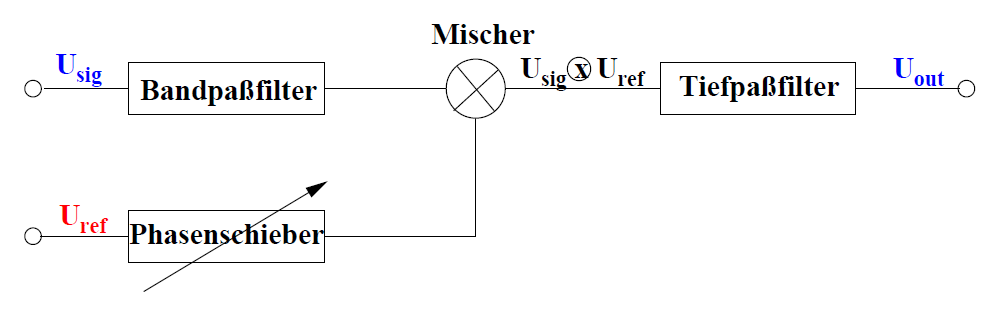
\includegraphics[width=\linewidth-70pt,height=\textheight-70pt,keepaspectratio]{content/images/schematischerAufbau.png}
	\caption{Schematischer Aufbau des Lock-In-Verstärkers\cite{V303}}
	\label{fig:schematischerAufbau}
\end{figure}

\noindent Betrachtet man eine Sinusspannung der Form $U_.{sig}=U_.0\text{sin}(\omega t)$ als Eingangssignal, so ergibt sich mit einer Sinusspannung $U_.{ref}=U_.1\text{sin}(\omega t+\phi_.0)$ als Referenzsignal für $U_.{out}$:
\begin{equation}
U_.{out} = \frac{U_.0U_.1}{2}\text{cos}(\phi)\text{.}
\end{equation}
Für eine Rechteckspannung kann $U_{ref}$ als Fourierreihe angenähert werden:
\begin{equation}
U_.{ref} = \frac{4U_.1}{\pi}\sum_{n=1}^{\infty}\frac{\text{sin}((2n-1)\omega t)}{2n-1}\text{.}
\end{equation}
Nach Multiplikation mit $U_.{sig}$ und Integration über $t$ ergibt sich für die Ausgangsspannung:
\begin{equation}
U_.{out} = \frac{2U_.0U_.1}{\pi}\text{cos}(\phi)\text{.}
\end{equation}